
\chapter{Vysledky prace}

V tejto kapitole zhrnieme vysledky ktore nasa praca dosiahla.

Uz v predchadzajucich kappitolach sme sa stretli s niekolkymi prikladmi, napriklad ako si
program poradil s vkladanim do hairpinu - obrazok \ref{obr:insert_circle_hairpin}.

Na dalsom (obrazok \ref{obr:delete_insert_multibranch}) simulujeme mazanie s naslednym vkladanim,
teda 2 k sebe inverzne operacie. Po zmazaní bazovych parov na hornej vetve molekuly, sa nam vsetky
neparove bazy zliali a vytvorili jednu loop. Nasledne po opatovnom vlozeni bazovych parov (pre lepsie
zviditelnenie sme ich oznacili "I"), vznikla struktura velmi podobna predchadzajucej.

Obrazok ma za ciel ukazat, ze vieme znovu nakreslit povodnu strukturu iba s malymi zmenamy v pozicii
nukleotidov (vysledne loopy su trochu plytsie ako povodne).

Rovnako obrazok \ref{obr:delete_insert_multibranch_loop} rekonstruuje vetvenie sa stromu. Ako je vidiet,
v tomto obrazku je uz viac rozdielov, vychylenie je celkom badatelne.

Na takto malych castiach bez velkych vetveni nam ani taketo zmeny nevadia. Pri velkych molekulach
ako ukazeme neskor problemy nastavaju.

\begin{figure}[H]
  \begin{subfigure}{0.3\textwidth}
%trim=left bottom right top
    \fbox{
\includegraphics[clip, trim=1cm 21cm 14cm 2.5cm, width=0.85\textwidth]{../img/alg-insert/2/multibranch-beg}}
  \end{subfigure}
  \begin{subfigure}{0.3\textwidth}
%trim=left bottom right top
    \fbox{\includegraphics[clip, trim=1cm 21cm 14cm 2.5cm, width=0.85\textwidth]{../img/alg-insert/2/multibranch-del}}
  \end{subfigure}
  \begin{subfigure}{0.3\textwidth}
%trim=left bottom right top
    \fbox{\includegraphics[clip, trim=1cm 21cm 14cm 2.5cm, width=0.85\textwidth]{../img/alg-insert/2/multibranch-del-ins}}
  \end{subfigure}
  \caption{Inverzne operacie: rekonstrukcia stemu}
  \label{obr:delete_insert_multibranch}
\end{figure}


\begin{figure}[H]
  \begin{subfigure}{0.3\textwidth}
%trim=left bottom right top
    \fbox{
\includegraphics[clip, trim=0 0 0 3cm, width=0.85\textwidth]{../img/alg-insert/3/multibranch-beg}}
  \end{subfigure}
  \begin{subfigure}{0.3\textwidth}
%trim=left bottom right top
    \fbox{\includegraphics[clip, trim=0 0 0 3cm, width=0.85\textwidth]{../img/alg-insert/3/multibranch-del}}
  \end{subfigure}
  \begin{subfigure}{0.3\textwidth}
%trim=left bottom right top
    \fbox{\includegraphics[clip, trim=0 0 0 3cm, width=0.85\textwidth]{../img/alg-insert/3/multibranch-del-ins}}
  \end{subfigure}
  \caption{Inverzne operacie: rekonstrukcia multibranch loop}
  \label{obr:delete_insert_multibranch_loop}
\end{figure}




